\documentclass[journal=jctcce,a4paper]{achemso}

\usepackage[utf8]{inputenc}
\usepackage[T1]{fontenc}
\usepackage{csquotes}
\usepackage{siunitx}
\usepackage{cleveref}
\usepackage{listings}
\MakeOuterQuote{"}

\lstset{
  basicstyle=\ttfamily,
  showstringspaces=false,
  keywordstyle=\bfseries,
  keywordstyle=[2]\bfseries,
  numbers=left,
  numberstyle=\tiny,
  frame=single,
  literate = {-}{-}1,
  breaklines = true,
  breakatwhitespace = true,
  breakindent = 0pt,
  postbreak=\mbox{$\hookrightarrow$\space},
}
\lstdefinelanguage{OpenMolcas}{
  sensitive=false,
  moredelim=[l][keywordstyle]{\&},
  moredelim=*[l][keywordstyle2]{>},
  morecomment=[f][commentstyle][0]{*},
  morecomment=[l]{//},
  morecomment=[s]{/*}{*/},
}

\newcommand{\lastname}[1]{#1}
\newcommand{\orcid}[1]{\relax}

\title{OpenMolcas--MRCC Interface for High-Accuracy Coupled-Cluster Calculations}

\def\affilUniNameA{HPQC Labs, Waterloo N2T 2K9 Ontario, Canada}

\author{Nike \lastname{Dattani}\orcid{0000-0001-5667-3632}}
  \affiliation{\affilUniNameA}
  \email{nike@hpqc.org}

\author{Jaafar \lastname{Mehrez}\orcid{0000-0002-4784-7052}}
  \affiliation{\affilUniNameA}
  \email{jaafar@hpqc.org}

\begin{document}

\sloppy\frenchspacing
\maketitle

%%%%%% BEGIN CONTRIBUTION %%%%%%%%%%%%%%%%%%%%%%%%%%%%%%%%%%%%%%%%%%%%%%%%%%%%%%

\section*{Abstract}

An interface between OpenMolcas and the MRCC program has been implemented, enabling the export of 
active-space integrals in the \texttt{fort.55} format required by MRCC for high-level coupled-cluster and 
configuration-interaction calculations.

\section*{Introduction}

The MRCC program offers state-of-the-art coupled-cluster (CC) and configuration-interaction (CI) methods, 
including arbitrary-order iterative and perturbative CC approaches.\cite{Kallay2020} The present interface bridges 
OpenMolcas and MRCC by enabling the export of active-space integrals in the \texttt{fort.55} format required by MRCC, 
thereby granting OpenMolcas users access to high-level CC methods.

\section*{Main body}

\begin{figure}
\centering
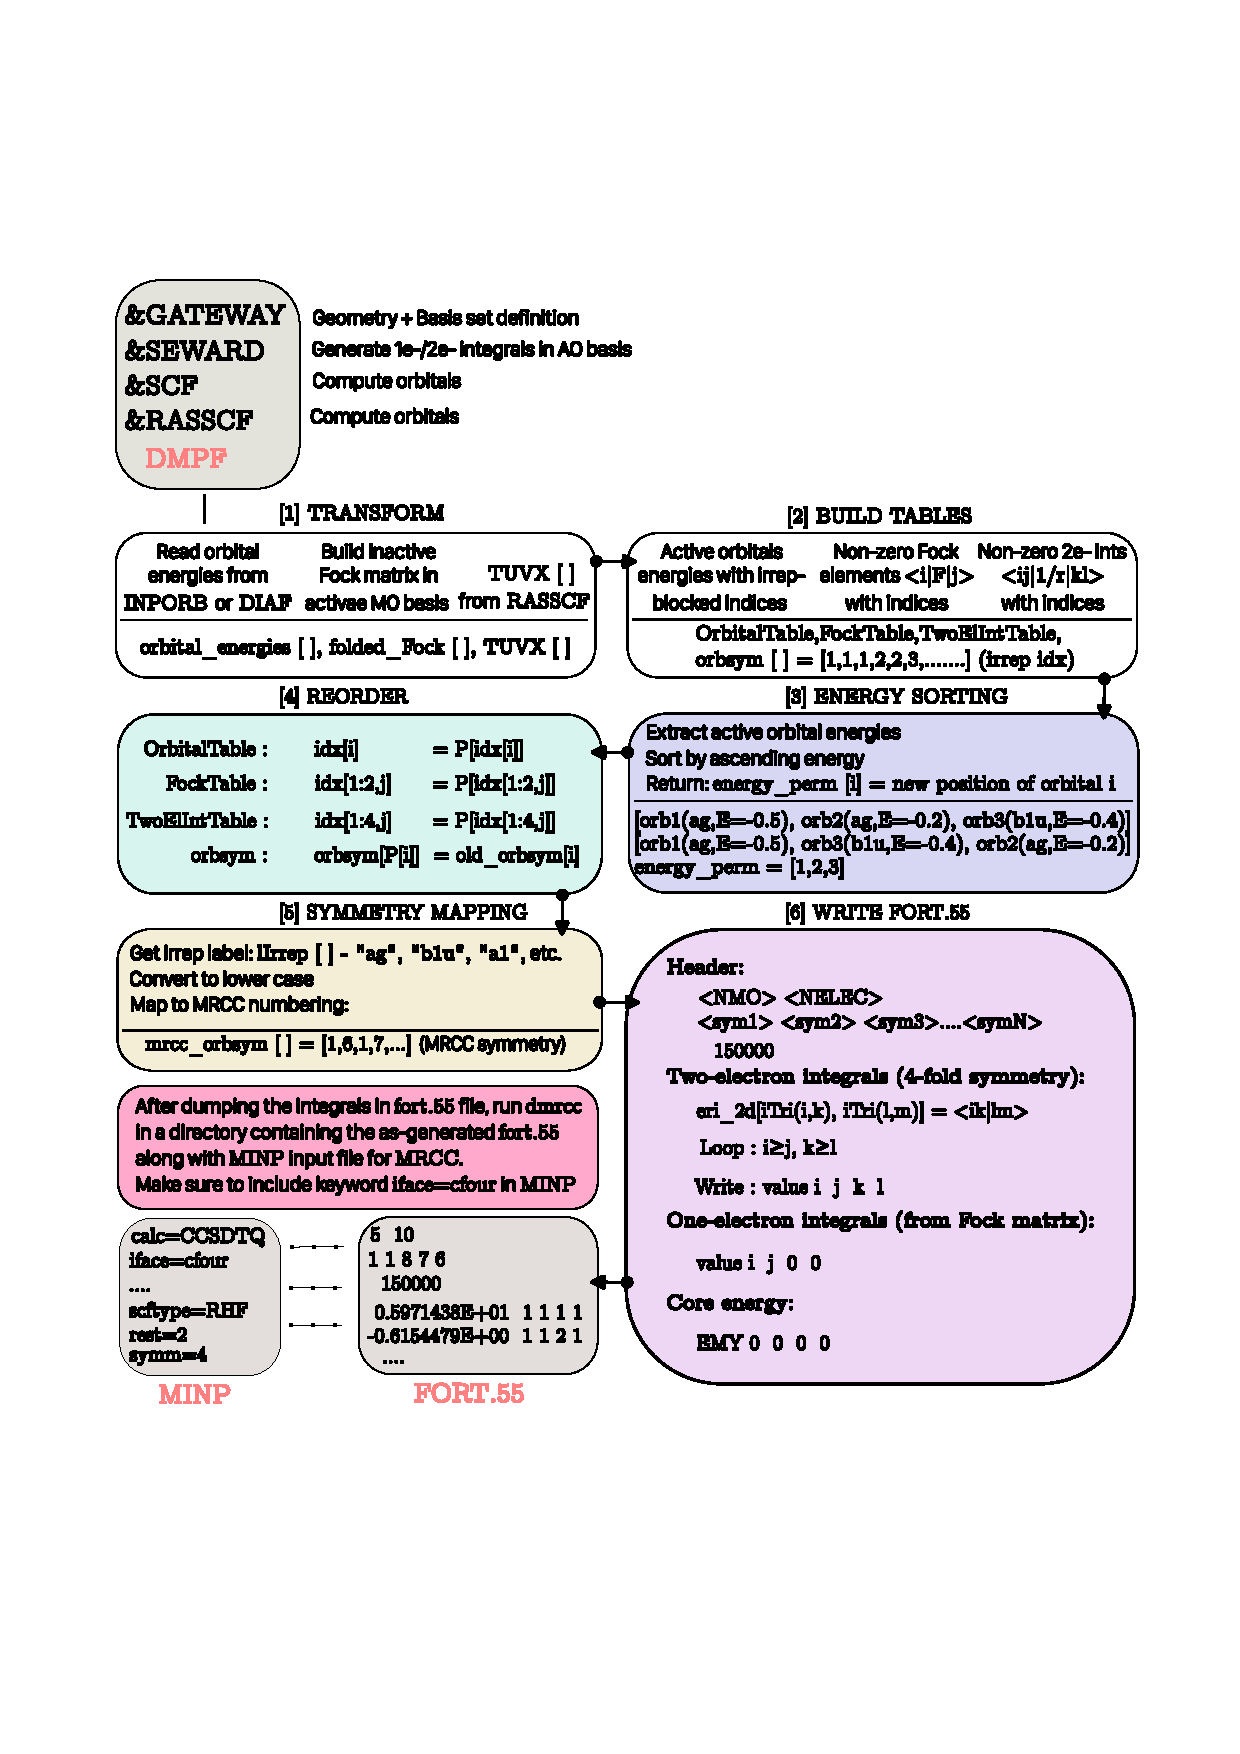
\includegraphics[width=\textwidth,trim=40pt 120pt 40pt 130pt, clip=true]{figures/molcas-mrcc.pdf}
\caption{Workflow of the OpenMolcas--MRCC interface. The \texttt{RASSCF} module generates a \texttt{fort.55} integral 
file using \texttt{DMPF} keyword, that is subsequently read by MRCC using \texttt{iface=cfour}.}
\label{fig:workflow}
\end{figure}

The interface is implemented within the \texttt{RASSCF} module and is activated by the dedicated \texttt{DMPF} 
keyword, which produces the MRCC-compatible \texttt{fort.55} file and quits in a clean manner without running a 
CI or CASSCF calculation (\cref{fig:workflow}). This is separate from the existing \texttt{DMPO} keyword, which 
retains its original role of dumping \texttt{FCIDUMP} files as in the case of the OpenMolcas--NECI and 
OpenMolcas--DICE interfaces.\cite{LiManni2023} The \texttt{fort.55} file is registered 
in the module file registry, so the OpenMolcas wrapper automatically copies it from the scratch directory to the 
user's output directory.
The \texttt{fort.55} format differs from the standard FCIDUMP in that active orbitals are reordered from Molcas 
irrep-grouped ordering into ascending-energy ordering, as required by MRCC. Two-electron integrals are written 
in 4-fold format ($i \ge j,\; k \ge l$), one-electron integrals are taken from the Fock matrix, and the core 
energy is appended. Symmetry labels are mapped from the Molcas irrep numbering to the MRCC convention for the 
supported point groups $C_1$, $C_i$, $C_s$, $C_2$, $C_{2v}$, $C_{2h}$, $D_2$, and $D_{2h}$.

To verify the correctness of the interface, a benchmark was performed on a neon atom in $D_{2h}$ symmetry with the 
6-31G basis set. The CCSDTQ energy obtained from MRCC using the OpenMolcas-generated \texttt{fort.55} file 
($-128.589\,793\,424\,699~E_\mathrm{h}$) is identical to that from MRCC's own integral generation, confirming 
faithful transfer of the Hamiltonian.

\section*{Conclusions}

The OpenMolcas--MRCC interface extends the capabilities of OpenMolcas by providing seamless access to high-level 
CC methods in MRCC.

\section*{Acknowledgements}


\section*{Supporting information}

{\setstretch{1}

The following input file generates a \texttt{fort.55} integral file for a neon atom in $D_{2h}$ symmetry with the 
6-31G basis set (test \texttt{additional/486}).

\begin{lstlisting}[language=OpenMolcas,caption={OpenMolcas input for generating a \texttt{fort.55} file.},label=lst:mrcc-inp]
&GATEWAY
  coord
    1
    angstrom
    Ne  0.000000  0.000000  0.000000
  basis = 6-31G

&SEWARD

&SCF
  Threshold = 0.5D-14 0.5D-14 0.5D-14 0.5D-14

&RASSCF
  OutOrbitals = CANOnical
  nActEl = 10 0 0
  Ras2 = 3 2 2 0 2 0 0 0
  DMPF
\end{lstlisting}

After running OpenMolcas, the MRCC calculation can be launched by executing \texttt{dmrcc} in the same directory 
containing the generated \texttt{fort.55} file and the MRCC input file \texttt{MINP}, make sure to include the 
keyword \texttt{iface=cfour}. The corresponding MRCC \texttt{MINP} for a CCSDTQ calculation reads:

\begin{lstlisting}[language=bash,caption={MRCC \texttt{MINP} input file.},label=lst:mrcc-minp]
iface=cfour
calc=CCSDTQ
cctol=10
ccmaxit=999
scftype=RHF
\end{lstlisting}

}

%%%%%% END CONTRIBUTION %%%%%%%%%%%%%%%%%%%%%%%%%%%%%%%%%%%%%%%%%%%%%%%%%%%%%%%%

\bibliography{bibliography}

\end{document}
